\documentclass[border=3pt, tikz, convert]{standalone}
\usepackage{amsmath}
\usetikzlibrary{arrows, positioning, arrows.meta, fit, shapes}
\newcommand{\empt}[2]{$#1^{(#2)}$}

\begin{document}

% State space model
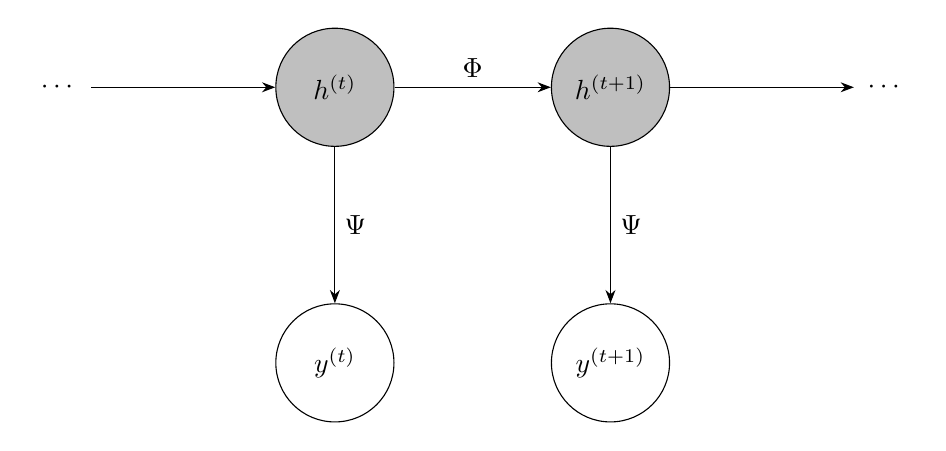
\begin{tikzpicture}[node distance=3.5cm]
    % Nodes
    \node[circle] (prev) {$\cdots$};
    \node[draw, fill=gray!50, circle, right of=prev, minimum size=1.5cm] (current state) {$h^{(t)}$};
    \node[draw, fill=gray!50, circle, right of=current state, minimum size=1.5cm] (next state) {$h^{(t+1)}$};
    \node[circle, right of=next state] (dots) {$\cdots$};
    \node[draw, circle, below of=current state, minimum size=1.5cm] (current obs) {$y^{(t)}$};
    \node[draw, circle, below of=next state, minimum size=1.5cm] (next obs) {$y^{(t+1)}$};

    % Connections
    \draw [arrows = {-Stealth[scale=1]}] (prev) -- (current state);
    \draw [arrows = {-Stealth[scale=1]}] (current state) -- (next state)
    	node[midway, above] {$\Phi$};
    \draw [arrows = {-Stealth[scale=1]}] (next state) -- (dots);
    \draw [arrows = {-Stealth[scale=1]}] (current state) -- (current obs)
    	node[midway, right] {$\Psi$};
    \draw [arrows = {-Stealth[scale=1]}] (next state) -- (next obs)
        	node[midway, right] {$\Psi$};
\end{tikzpicture}

% State space model with exogenous vairables
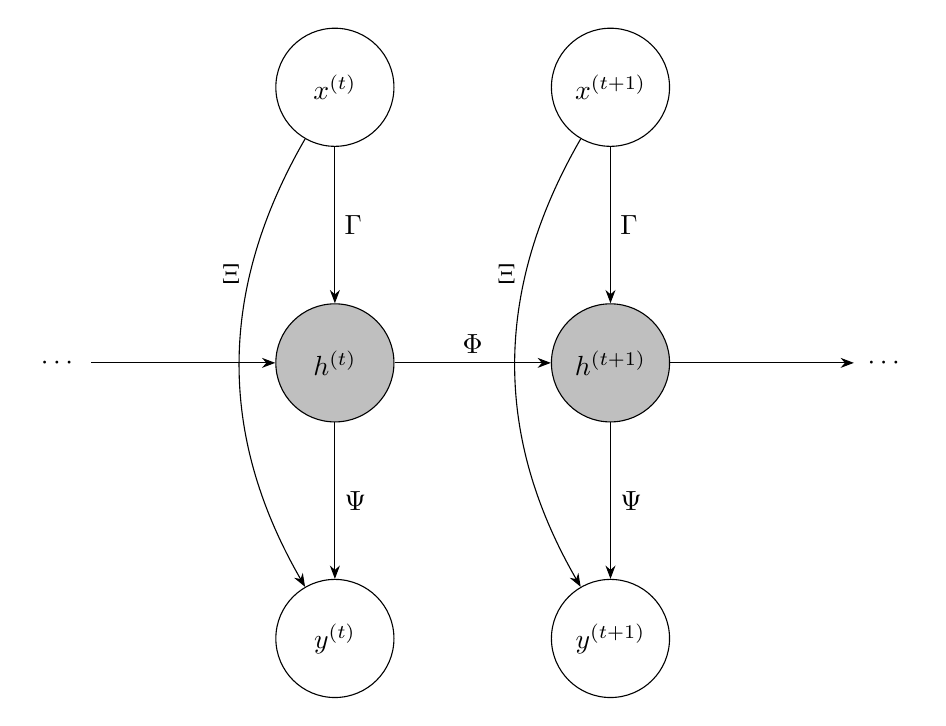
\begin{tikzpicture}[node distance=3.5cm]
    % Nodes
    \node[circle] (prev) {$\cdots$};
    \node[draw, fill=gray!50, circle, right of=prev, minimum size=1.5cm] (current state) {$h^{(t)}$};
    \node[draw, fill=gray!50, circle, right of=current state, minimum size=1.5cm] (next state) {$h^{(t+1)}$};
    \node[draw, circle, above of=current state, minimum size=1.5cm] (current exo) {$x^{(t)}$};
    \node[draw, circle, above of=next state, minimum size=1.5cm] (next exo) {$x^{(t+1)}$};
    \node[circle, right of=next state] (dots) {$\cdots$};
    \node[draw, circle, below of=current state, minimum size=1.5cm] (current obs) {$y^{(t)}$};
    \node[draw, circle, below of=next state, minimum size=1.5cm] (next obs) {$y^{(t+1)}$};

    % Connections
    \draw [arrows = {-Stealth[scale=1]}] (prev) -- (current state);
    \draw [arrows = {-Stealth[scale=1]}] (current state) -- node[midway, above] {$\Phi$} (next state);
    \draw [arrows = {-Stealth[scale=1]}] (next state) -- (dots);
    \draw [arrows = {-Stealth[scale=1]}] (current exo) -- node[midway, right] {$\Gamma$} (current state);
    \draw [arrows = {-Stealth[scale=1]}] (next exo) -- node[midway, right] {$\Gamma$} (next state);
    \draw [arrows = {-Stealth[scale=1]}] (current state) -- node[midway, right] {$\Psi$} (current obs);
    \draw [arrows = {-Stealth[scale=1]}] (next state) -- node[midway, right] {$\Psi$} (next obs);
    \draw [arrows = {-Stealth[scale=1]}](current exo) to [bend right=30] node[pos=0.3,left]{$\Xi$} (current obs);
    \draw [arrows = {-Stealth[scale=1]}](next exo) to [bend right=30] node[pos=0.3,left]{$\Xi$} (next obs);
\end{tikzpicture}

% Simple RNN
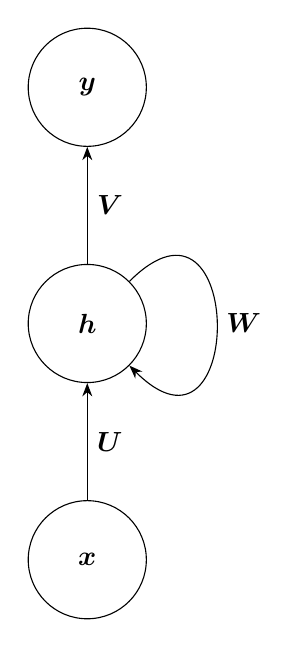
\begin{tikzpicture}[node distance=3cm]
    % Nodes
    \node[draw, circle, minimum size=1.5cm] (hidden) {$\boldsymbol{h}$};  
    \node[draw, circle, below of=hidden, minimum size=1.5cm] (input) {$\boldsymbol{x}$};
    \node[draw, circle, above of=hidden, minimum size=1.5cm] (out) {$\boldsymbol{y}$};

    % Connections
    \draw [arrows = {-Stealth[scale=1]}] (input) to node[midway, right] {$\boldsymbol{U}$} (hidden);
    \draw [arrows = {-Stealth[scale=1]}] (hidden) to[out = 45, in=315, looseness=5] node[midway, right] {$\boldsymbol{W}$} (hidden);
    \draw [arrows = {-Stealth[scale=1]}] (hidden) to node[midway, right] {$\boldsymbol{V}$} (out);
\end{tikzpicture}

% unfolded RNN

\begin{tikzpicture}[node distance=3.5cm]
	
    %% folded
    % Nodes
    \node[draw, circle, minimum size=1.5cm] (hidden) {$\boldsymbol{h}$};  
    \node[draw, circle, below of=hidden, minimum size=1.5cm] (input) {$\boldsymbol{x}$};
    \node[draw, circle, above of=hidden, minimum size=1.5cm] (out) {$\boldsymbol{y}$};

    % Connections
    \draw [arrows = {-Stealth[scale=1]}] (input) to node[midway, right] {$\boldsymbol{U}$} (hidden);
    \draw [arrows = {-Stealth[scale=1]}] (hidden) to[out = 45, in=315, looseness=5] node[midway, right] {$\boldsymbol{W}$} (hidden);
    \draw [arrows = {-Stealth[scale=1]}] (hidden) to node[midway, right] {$\boldsymbol{V}$} (out);
    
    \node[circle, right of=hidden] (arrow) {\scalebox{3}{$\Rightarrow$}};

    %% Unfolded
    % Nodes
    \node[circle, right=0.3cm of arrow] (prev) {$\cdots$};
    \node[draw, circle, right =1cm of prev, minimum size=1.5cm] (hidden1) {$\boldsymbol{h}^{(t)}$};
    \node[draw, circle, right of=hidden1, minimum size=1.5cm] (hidden2) {$\boldsymbol{h}^{(t+1)}$};
    \node[draw, circle, above of=hidden1, minimum size=1.5cm] (out1) {$\boldsymbol{y}^{(t)}$};
    \node[draw, circle, above of=hidden2, minimum size=1.5cm] (out2) {$\boldsymbol{y}^{(t+1)}$};
    \node[circle, right =1cm of hidden2] (dots) {$\cdots$};
    \node[draw, circle, below of=hidden1, minimum size=1.5cm] (input1) {$\boldsymbol{x}^{(t)}$};
    \node[draw, circle, below of=hidden2, minimum size=1.5cm] (input2) {$\boldsymbol{x}^{(t+1)}$};

    % Connections
    \draw [arrows = {-Stealth[scale=1]}] (prev) -- (hidden1);
    \draw [arrows = {-Stealth[scale=1]}] (hidden1) -- node[midway, above] {$\boldsymbol{W}$} (hidden2);
    \draw [arrows = {-Stealth[scale=1]}] (hidden2) -- (dots);
    \draw [arrows = {-Stealth[scale=1]}] (hidden1) to node[midway, right] {$\boldsymbol{V}$} (out1);
    \draw [arrows = {-Stealth[scale=1]}] (hidden2) to node[midway, right] {$\boldsymbol{V}$} (out2);
    \draw [arrows = {-Stealth[scale=1]}] (input1) to node[midway, right] {$\boldsymbol{U}$} (hidden1);
    \draw [arrows = {-Stealth[scale=1]}] (input2) to node[midway, right] {$\boldsymbol{U}$} (hidden2);
\end{tikzpicture}

% LSTM

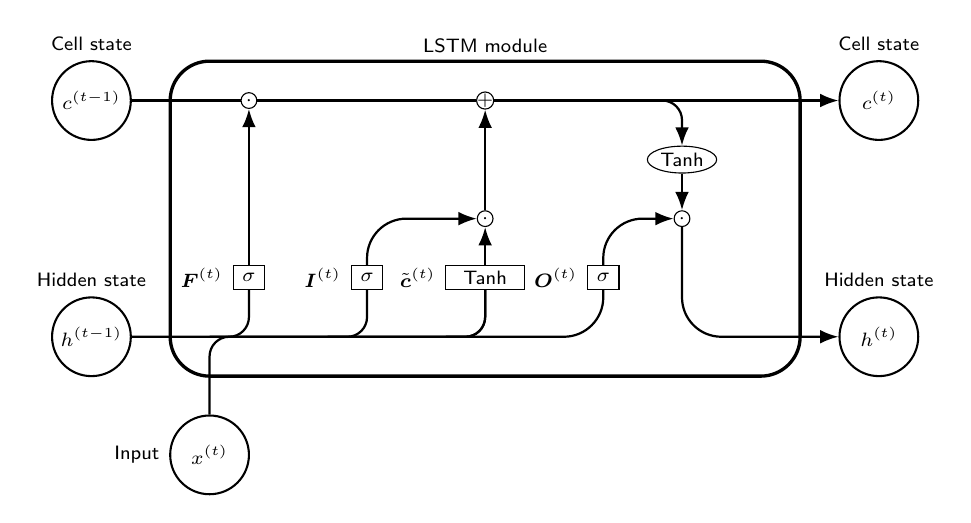
\begin{tikzpicture}[
    % GLOBAL CFG
    font=\sf \scriptsize,
    >=LaTeX,
    % Styles
    cell/.style={% For the main box
        rectangle, 
        rounded corners=5mm, 
        draw,
        very thick,
        },
    operator/.style={%For operators like +  and  x
        circle,
        draw,
        inner sep=-0.5pt,
        minimum height =.2cm,
        },
    function/.style={%For functions
        ellipse,
        draw,
        inner sep=1pt
        },
    ct/.style={% For external inputs and outputs
        circle,
        draw,
        line width = .75pt,
        minimum width=1cm,
        inner sep=1pt,
        },
    gt/.style={% For internal inputs
        rectangle,
        draw,
        minimum width=4mm,
        minimum height=3mm,
        inner sep=1pt
        },
    mylabel/.style={% something new that I have learned
        font=\scriptsize\sffamily
        },
    ArrowC1/.style={% Arrows with rounded corners
        rounded corners=.25cm,
        thick,
        },
    ArrowC2/.style={% Arrows with big rounded corners
        rounded corners=.5cm,
        thick,
        },
    ]

%Start drawing the thing...    
    % Draw the cell: 
    \node [cell, minimum height =4cm, minimum width=8cm] at (0,0){} ;
    \node at (0, 2.2) {LSTM module};

    % Draw inputs named ibox#
    \node [gt, label={[mylabel]left:$\boldsymbol{F}^{(t)}$}] (ibox1) at (-3,-0.75) {$\sigma$};
    \node [gt, label={[mylabel]left:$\boldsymbol{I}^{(t)}$}] (ibox2) at (-1.5,-0.75) {$\sigma$};
    \node [gt, label={[mylabel]left:$\tilde{\boldsymbol{c}}^{(t)}$}, minimum width=1cm] (ibox3) at (0,-0.75) {Tanh};
    \node [gt, label={[mylabel]left:$\boldsymbol{O}^{(t)}$}] (ibox4) at (1.5,-0.75) {$\sigma$};

   % Draw opérators   named mux# , add# and func#
    \node [operator] (mux1) at (-3,1.5) {$\cdot$};
    \node [operator] (add1) at (0,1.5) {+};
    \node [operator] (mux2) at (0,0) {$\cdot$};
    \node [operator] (mux3) at (2.5,0) {$\cdot$};
    \node [function] (func1) at (2.5,0.75) {Tanh};

    % Draw External inputs? named as basis c,h,x
    \node[ct, label={[mylabel]Cell state}] (c) at (-5,1.5) {\empt{c}{t-1}};
    \node[ct, label={[mylabel]Hidden state}] (h) at (-5,-1.5) {\empt{h}{t-1}};
    \node[ct, label={[mylabel]left:Input}] (x) at (-3.5,-3) {\empt{x}{t}};

    % Draw External outputs? named as basis c2,h2,x2
    \node[ct, label={[mylabel]Cell state}] (c2) at (5,1.5) {\empt{c}{t}};
    \node[ct, label={[mylabel]Hidden state}] (h2) at (5,-1.5) {\empt{h}{t}};


% Start connecting all.
    %Intersections and displacements are used. 
    % Drawing arrows    
    \draw [->, ArrowC1] (c) -- (mux1) -- (add1) -- (c2);

    % Inputs
    \draw [ArrowC2] (h) -| (ibox4);
    \draw [ArrowC1] (h -| ibox1)++(-0.5,0) -| (ibox1); 
    \draw [ArrowC1] (h -| ibox2)++(-0.5,0) -| (ibox2);
    \draw [ArrowC1] (h -| ibox3)++(-0.5,0) -| (ibox3);
    \draw [ArrowC1] (x) -- (x |- h)-| (ibox3);

    % Internal
    \draw [->, ArrowC2] (ibox1) -- (mux1);
    \draw [->, ArrowC2] (ibox2) |- (mux2);
    \draw [->, ArrowC2] (ibox3) -- (mux2);
    \draw [->, ArrowC2] (ibox4) |- (mux3);
    \draw [->, ArrowC2] (mux2) -- (add1);
    \draw [->, ArrowC1] (add1 -| func1)++(-0.5,0) -| (func1);
    \draw [->, ArrowC2] (func1) -- (mux3);

    %Outputs
    \draw [->, ArrowC2] (mux3) |- (h2);

\end{tikzpicture}

% Deep RNN

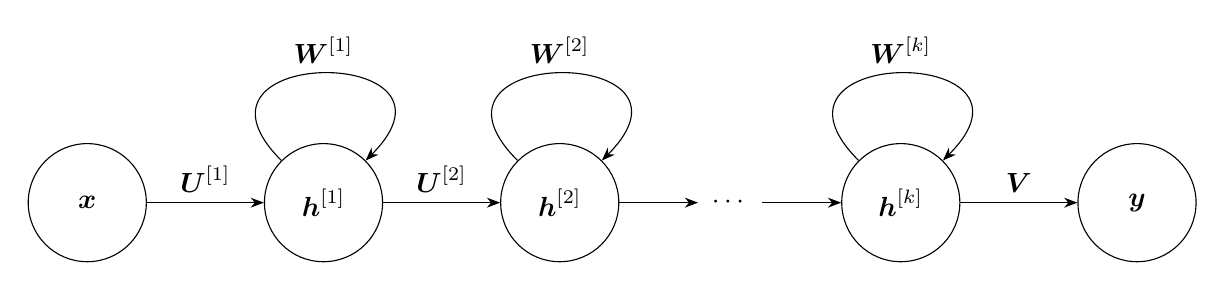
\begin{tikzpicture}[node distance=3cm]
    % Nodes
    \node[draw, circle, minimum size=1.5cm] (input) {$\boldsymbol{x}$};  
    \node[draw, circle, right of=input, minimum size=1.5cm] (hidden1) {$\boldsymbol{h}^{[1]}$};
    \node[draw, circle, right of=hidden1, minimum size=1.5cm] (hidden2) {$\boldsymbol{h}^{[2]}$};
    \node[circle, right=1cm of hidden2] (dots) {$\cdots$};
    \node[draw, circle, right=1cm of dots, minimum size=1.5cm] (hidden3) {$\boldsymbol{h}^{[k]}$};
    \node[draw, circle, right of=hidden3, minimum size=1.5cm] (output) {$\boldsymbol{y}$};

    % Connections
    \draw [arrows = {-Stealth[scale=1]}] (input) to node[midway, above] {$\boldsymbol{U}^{[1]}$} (hidden1);
    \draw [arrows = {-Stealth[scale=1]}] (hidden1) to node[midway, above] {$\boldsymbol{U}^{[2]}$} (hidden2);
    \draw [arrows = {-Stealth[scale=1]}] (hidden2) to (dots);
    \draw [arrows = {-Stealth[scale=1]}] (dots) to (hidden3);
    \draw [arrows = {-Stealth[scale=1]}] (hidden3) to node[midway, above] {$\boldsymbol{V}$} (output);
    \draw [arrows = {-Stealth[scale=1]}] (hidden1) to[out = 135, in=45, looseness=5] node[midway, above] {$\boldsymbol{W}^{[1]}$} (hidden1);
    \draw [arrows = {-Stealth[scale=1]}] (hidden2) to[out = 135, in=45, looseness=5] node[midway, above] {$\boldsymbol{W}^{[2]}$} (hidden2);
    \draw [arrows = {-Stealth[scale=1]}] (hidden3) to[out = 135, in=45, looseness=5] node[midway, above] {$\boldsymbol{W}^{[k]}$} (hidden3);
    %\draw [arrows = {-Stealth[scale=1]}] (hidden) to node[midway, right] {$\boldsymbol{V}$} (out);
\end{tikzpicture}



\end{document}